\documentclass[11pt]{article}

\usepackage[margin=1in]{geometry}
\usepackage{times}
\usepackage{graphicx}
\usepackage{amsmath}
\usepackage{amssymb}
\usepackage{hyperref}
\usepackage{cite}
\usepackage{setspace}
\usepackage{titlesec}

\onehalfspacing
\hypersetup{colorlinks=true, linkcolor=black, citecolor=black, urlcolor=blue}

\titleformat{\section}{\normalfont\large\bfseries}{\thesection.}{0.5em}{}
\titleformat{\subsection}{\normalfont\normalsize\bfseries}{\thesubsection.}{0.5em}{}

\begin{document}

% ================= TITLE PAGE =================
\begin{titlepage}
\centering
\vspace*{3cm}

{\Huge \bfseries Recent Advancements in Biotechnology:\\[0.3cm] Stem Cell Therapy}

\vspace{1.5cm}
{\Large A Review Report}

\vspace{1cm}

% Placeholder for institutional or cover image
\begin{figure}[h]
\centering
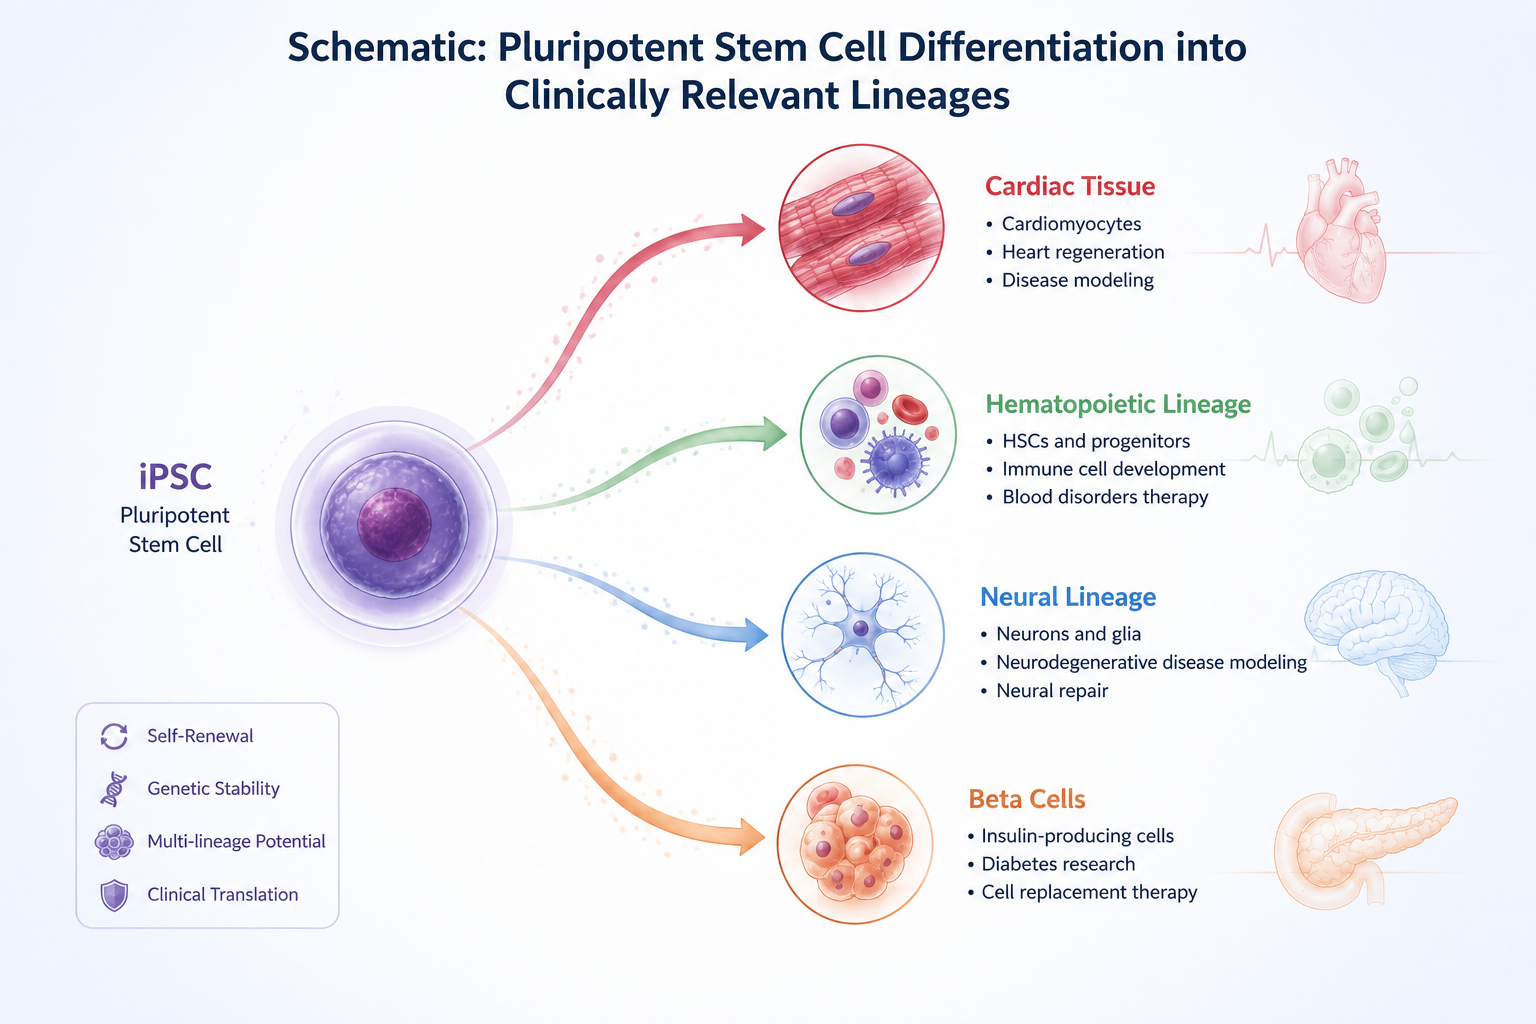
\includegraphics[width=0.7\textwidth]{Cover Image.png}
\caption{\textit{Cover illustration of stem cell differentiation / regenerative medicine concept}}
\end{figure}

\vspace{1cm}

\large
Prepared by: [Abu Henaf Rashid Ahmad Mufti] \\
Department: [Biotechnology Internship] \\
Institution: [CodeAlpha] \\
Date: July 13, 2026

\end{titlepage}

% ================= ABSTRACT =================
\section*{Abstract}
Stem cell therapy has moved from a mostly experimental discipline into one with an expanding catalogue of registered clinical trials, marketed products, and disease-specific programs. This report looks at where the field stands in 2025--2026, drawing on recent clinical trial landscape analyses, pluripotent stem cell trial reviews, and a phase I--II cardiac tissue trial. The main discussion covers three threads: the global scale and distribution of cell therapy trials, the clinical maturation of pluripotent stem cell-derived products across diabetes, neurological, and hematological applications, and a concrete case study of induced pluripotent stem cell (iPSC)-derived cardiac tissue in heart failure patients. I also cover autoimmune and inflammatory disease trials, where growth has been steady rather than explosive. Alongside the clinical progress, the report addresses persistent obstacles: immune rejection in allogeneic products, tumorigenicity risk from residual undifferentiated cells, manufacturing cost and scalability, and the ethical questions that still surround embryonic-derived lines and unproven commercial clinics. The report closes with a look at where the field seems to be heading -- allogeneic "off-the-shelf" products, combination therapies with gene editing, and tighter regulatory frameworks -- and argues that the next five years will likely be defined less by new discoveries and more by whether the field can translate its trial pipeline into approved, affordable therapies.

\vspace{0.5cm}
\noindent \textbf{Keywords:} stem cell therapy, induced pluripotent stem cells (iPSCs), regenerative medicine, cell therapy clinical trials, mesenchymal stem cells, heart failure

% ================= INTRODUCTION =================
\section{Introduction}

Stem cell biology sits at an odd point in its history right now. The core science, that certain cells can self-renew and differentiate into specialized lineages, has been understood for decades, but the translation of that science into approved, reliable therapies has taken far longer than early enthusiasm suggested it would. What has changed in the last two to three years is scale. Cell therapy clinical trials are no longer a handful of academic pilot studies; a recent global landscape analysis counted over ten thousand registered cell therapy trials worldwide, spanning autologous and allogeneic approaches, immune cell products, and classical stem cell types \cite{panoramic2026}.

This report focuses specifically on stem cell therapy as a subset of that broader cell therapy universe, meaning mesenchymal stem cells (MSCs), hematopoietic stem cells (HSCs), and pluripotent stem cells (both embryonic and induced). I want to trace what has actually moved from bench to bedside recently, not just what looks promising in a mouse model. The report draws on a 2025 update of pluripotent stem cell clinical trials \cite{kirkeby2025}, a large-scale trial landscape study \cite{panoramic2026}, an autoimmune-disease-specific trial analysis \cite{autoimmune2025}, and a phase I--II trial of iPSC-derived cardiac tissue reported in mid-2026 \cite{biovat2026}. Together these give a reasonably current picture of where stem cell therapy sits, rather than where it was five years ago.

% ================= BACKGROUND =================
\section{Background}

Stem cells are broadly classified by potency and origin. Embryonic stem cells (ESCs) are pluripotent, meaning they can give rise to any cell type of the three germ layers, but their use has always come with ethical friction tied to embryo destruction. Induced pluripotent stem cells (iPSCs), first generated by reprogramming adult somatic cells, sidestepped much of that controversy while retaining pluripotency, and they now account for a large share of new clinical trial activity. Adult stem cells, principally MSCs and HSCs, are multipotent, more limited in what they can become, but easier to source and have a much longer track record in the clinic, particularly HSCs in bone marrow transplantation.

The basic reprogramming efficiency for generating iPSCs from a starting population of somatic cells is still low relative to what a manufacturing process would ideally want. If $N_0$ is the number of somatic cells seeded and $N_r$ is the number of cells that successfully convert to a stable pluripotent state, the reprogramming efficiency $\eta$ is simply

\begin{equation}
\eta = \frac{N_r}{N_0} \times 100\%
\end{equation}

Efficiencies in the low single-digit percentages are still typical for standard viral or episomal reprogramming protocols, which is one of the practical reasons that scaling iPSC-derived products for large clinical trials remains harder than it sounds on paper.

Cell therapies are also distinguished by whether they are autologous (the patient's own cells, engineered or expanded and returned to the same patient) or allogeneic (cells from a donor, potentially manufactured at scale and used across many recipients). This distinction matters enormously for cost, immune compatibility, and regulatory pathway, and it comes up repeatedly in the discussion below.

% ================= MAIN DISCUSSION =================
\section{Recent Advancements in Biotechnology}

\subsection{The Scale of the Global Trial Landscape}

The clearest sign that stem cell therapy has matured as a field is simply the number of trials now underway. A 2026 quantitative landscape analysis identified 10,373 cell therapy clinical trials worldwide, with the United States leading at 3,563 trials and China close behind at 3,365 \cite{panoramic2026}. Within that total, mesenchymal stem cells accounted for 1,904 trials and hematopoietic stem cells for 1,550, while CAR-T and other immune cell therapies made up the largest single category at 2,409 trials \cite{panoramic2026}. What stands out here is not just the volume but the geographic concentration: two countries account for the clear majority of global activity, which has downstream effects on where manufacturing capacity, regulatory expertise, and cost structures develop first.

\begin{figure}[h]
\centering
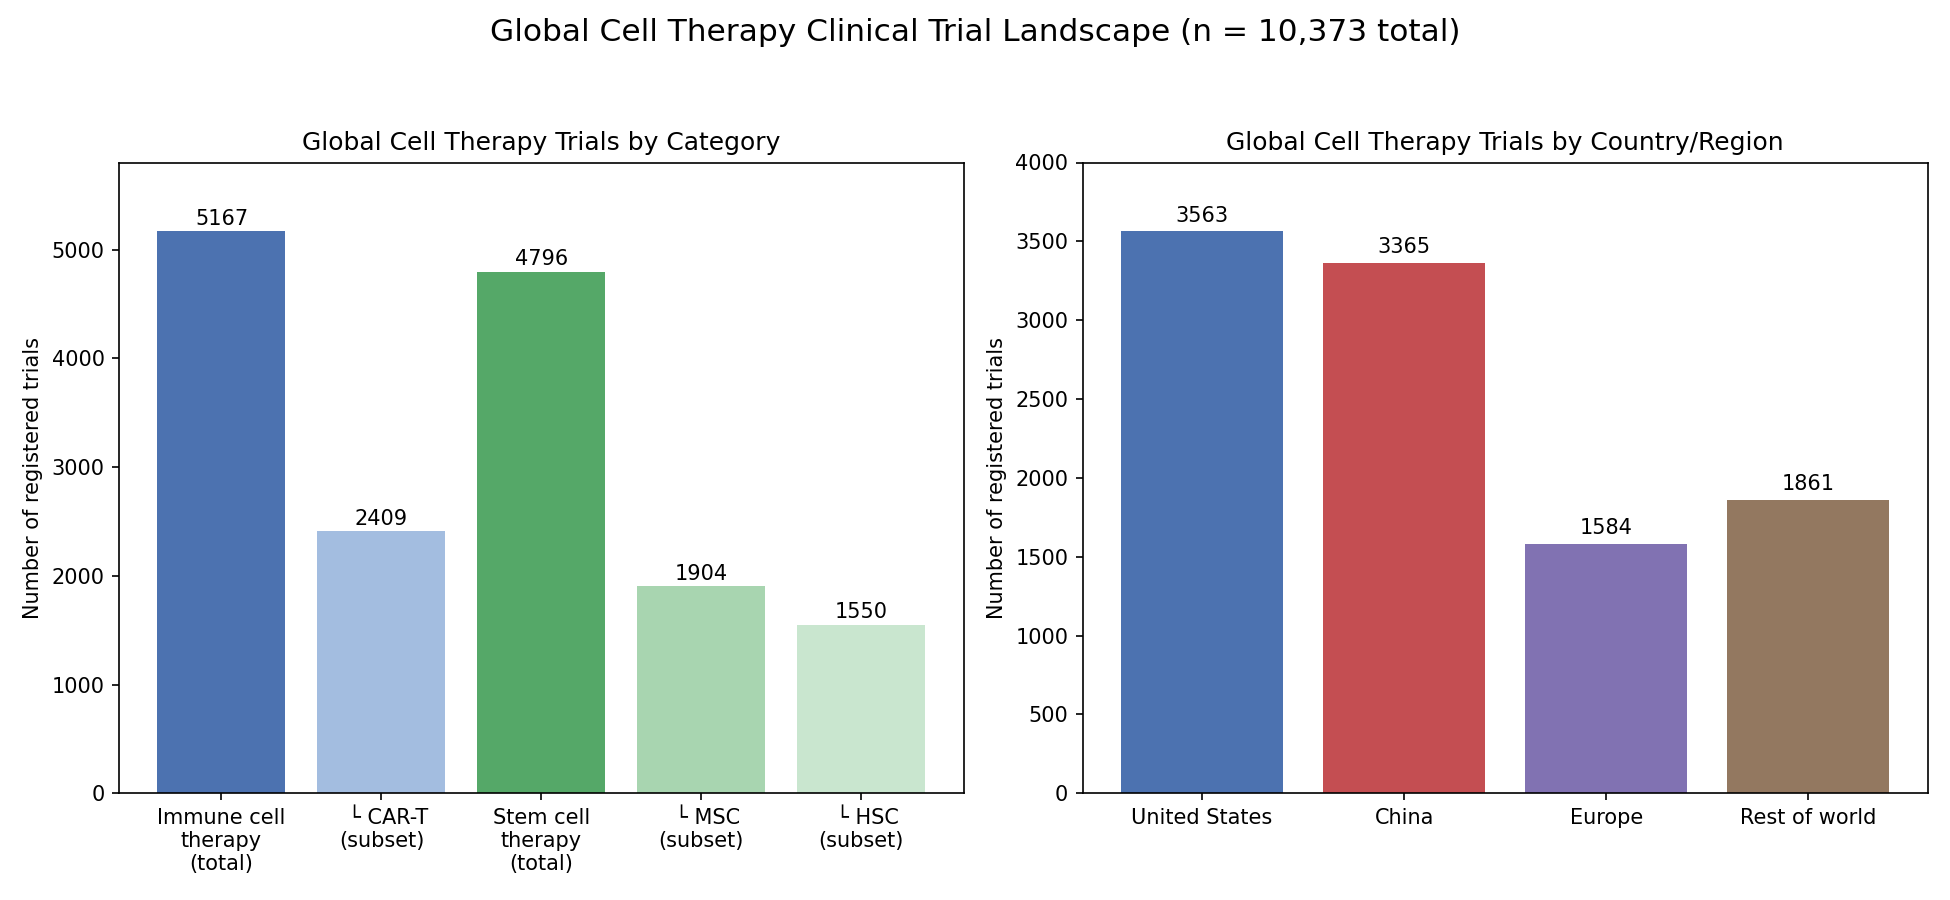
\includegraphics[width=0.95\textwidth]{trial_distribution_chart.png}
\caption{Bar chart of global cell therapy trial distribution by cell type and country (data from Frontiers in Pharmacology, 2026)}
\end{figure}

\subsection{Pluripotent Stem Cell-Derived Therapies in the Clinic}

Kirkeby and colleagues' 2025 update on pluripotent stem cell clinical trials gives a more granular view of what these trials are actually treating \cite{kirkeby2025}. Their review covers programs ranging from beta-cell replacement therapy for type 1 diabetes to allogeneic iPSC-derived natural killer (NK) and T-cell products for cancer, along with ongoing work in spinal cord injury repair. What I find notable about this review is less any single result and more the breadth: pluripotent stem cell products are no longer clustered around one or two flagship indications, they are spreading across endocrine, oncologic, and neurological applications simultaneously, which suggests the underlying manufacturing and differentiation platforms have become general-purpose enough to support multiple disease programs from the same technology base.

\subsection{A Concrete Clinical Result: iPSC-Derived Cardiac Tissue}

Reviews and landscape analyses are useful for seeing the shape of a field, but a single well-reported trial result is worth more for judging where the technology actually stands. The BioVAT-HF trial, an interim analysis published via Nature in mid-2026, transplanted a tissue allograft made from iPSC-derived cardiac cells into patients with advanced heart failure \cite{biovat2026}. At the three-month mark, the graft was associated with heart remuscularization along with measurable increases in wall thickness, ejection fraction, and patient-reported quality of life \cite{biovat2026}. This is a phase I--II interim result, so the sample size is necessarily small and durability past three months is not yet established, but it is one of the few instances where an iPSC-derived tissue product has shown a physiological effect on the organ it was designed to repair, not just safety and tolerability. If ejection fraction (EF) is used as the functional benchmark, the pre- to post-treatment change can be expressed simply as

\begin{equation}
\Delta EF = EF_{\text{post}} - EF_{\text{pre}}
\end{equation}

with the trial reporting a positive $\Delta EF$ at the three-month follow-up window, alongside improvements in wall thickness and quality-of-life scoring \cite{biovat2026}.

\subsection{Stem Cells in Autoimmune and Inflammatory Disease}

Away from oncology and cardiology, stem cell therapy has also been building a longer, quieter track record in autoimmune and inflammatory disease. An analysis of 1,136 stem cell trials drawn from the TrialTrove database traced the field's growth from roughly eleven new studies a year between 2000 and 2004 up to a peak of seventy-three new trials in 2019 \cite{autoimmune2025}. That is a meaningful growth curve, though it is worth noting the peak was several years before this current report, and the analysis does not claim the growth rate has continued unchanged since. Most of the activity here uses MSCs for their immunomodulatory properties rather than any capacity to regenerate tissue directly, which places these trials in a somewhat different mechanistic category from the pluripotent stem cell work discussed above.

\begin{figure}[h]
\centering
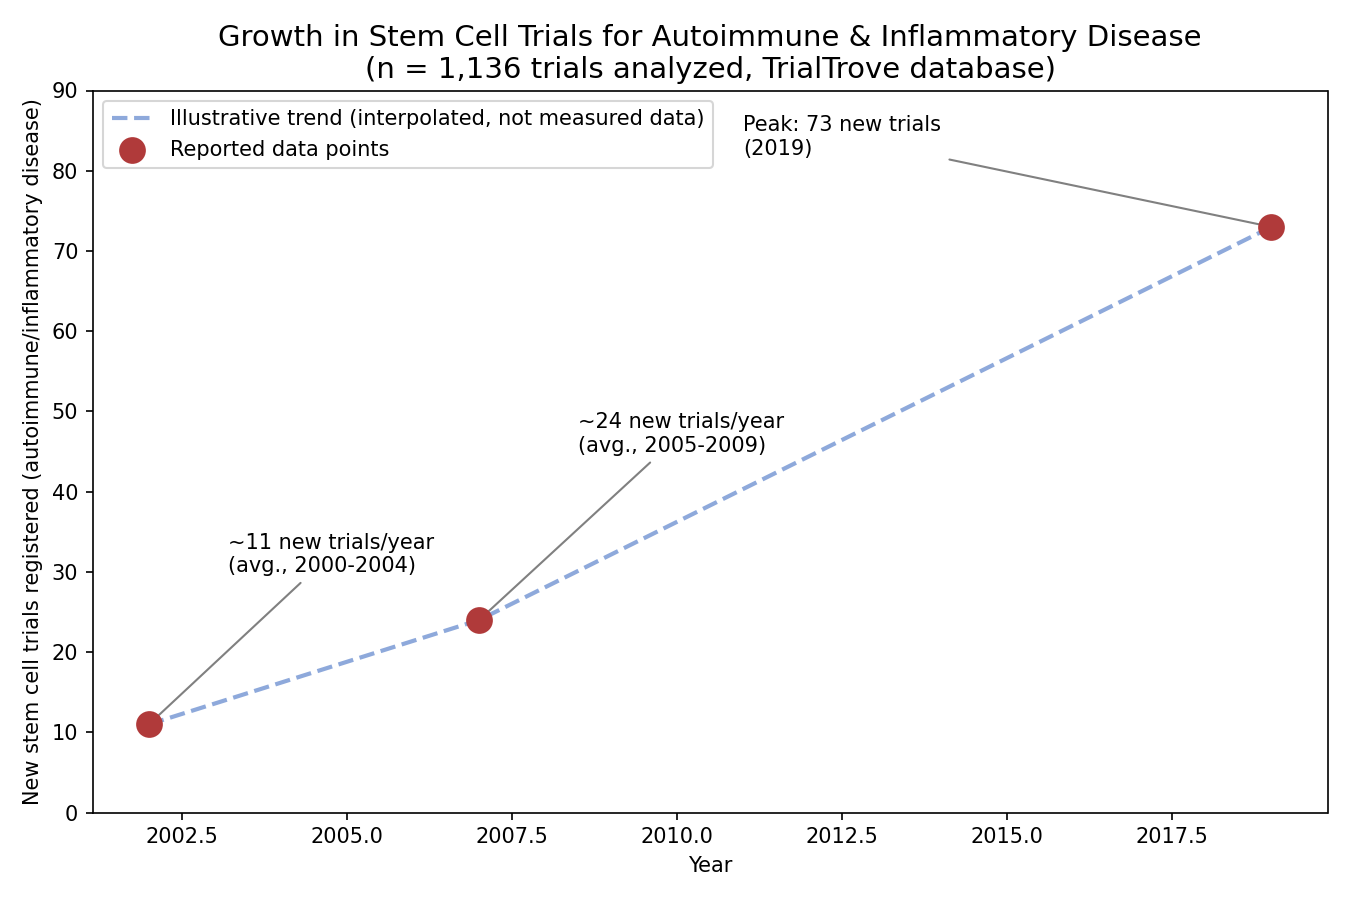
\includegraphics[width=0.9\textwidth]{trial_growth_timeline.png}
\caption{Timeline plot showing annual new stem cell trials in autoimmune/inflammatory disease, 2000--2019}
\end{figure}

\subsection{Marketed Products and Regulatory Trends}

Beyond trials still in progress, the panoramic landscape analysis also tracked marketed cell therapy products and regulatory trends \cite{panoramic2026}. The pattern that emerges is a slow but steady conversion of trial activity into approved products, concentrated heavily in hematological indications where HSC transplantation already has decades of regulatory precedent, and more recently in CAR-T products for blood cancers. Solid organ and tissue-regeneration indications, including the cardiac work described above, remain earlier in that conversion process, generally still in phase I or II rather than at the approval stage.

% ================= CHALLENGES =================
\section{Challenges and Ethical Considerations}

A few obstacles keep showing up across nearly all of these programs, regardless of cell type or indication.

\textbf{Immune rejection.} Allogeneic products, which is where much of the "off-the-shelf" commercial promise lies, still have to contend with host immune rejection unless the cells are engineered to be immune-evasive or the patient is immunosuppressed, which carries its own risks.

\textbf{Tumorigenicity.} Pluripotent stem cell products carry a specific risk that adult stem cell products mostly do not: any residual undifferentiated cells in the final product can, in principle, form teratomas. Manufacturing protocols now include purification steps aimed at this, but it remains a standing safety consideration in every iPSC trial design, including the cardiac tissue work described above.

\textbf{Manufacturing cost and scale.} Autologous products, by definition, cannot be mass-produced the way a small-molecule drug can. Each batch is essentially a custom manufacturing run for one patient, which keeps costs high. Allogeneic approaches promise to solve this, but they introduce the immune rejection problem back into the equation, so the field is really trading one difficulty for another rather than eliminating it.

\textbf{Ethical and regulatory questions.} Embryonic stem cell lines still carry ethical weight in some jurisdictions, even though iPSC technology has reduced reliance on them substantially. Separately, the rapid growth in trial numbers has been accompanied by a persistent problem of unproven, direct-to-consumer stem cell clinics operating outside formal trial structures, which the regulatory trend data reflects as an ongoing area of oversight concern rather than a solved issue \cite{panoramic2026}.

Taken together, these are not new problems, but the scale at which the field is now operating means their consequences are larger. A manufacturing bottleneck that was a minor inconvenience for a handful of academic trials becomes a real barrier when ten thousand trials are competing for specialized cleanroom capacity and trained cell-processing staff.

% ================= FUTURE DIRECTIONS =================
\section{Future Directions}

A few directions seem reasonably likely to shape the next several years. First, allogeneic "off-the-shelf" products, particularly iPSC-derived NK and T-cell therapies, are likely to keep expanding because they solve the manufacturing scalability problem even if they do not fully solve immune compatibility \cite{kirkeby2025}. Second, combination approaches pairing stem cell products with gene editing, so that immune evasion or targeting is engineered directly into the cell line rather than managed with drugs afterward, appear to be an increasingly common design choice in newer trial protocols. Third, given how concentrated trial activity currently is in the US and China \cite{panoramic2026}, it seems likely that manufacturing infrastructure and regulatory frameworks in other regions will need to catch up if global patient access is a genuine goal rather than an afterthought. Finally, results like the BioVAT-HF interim analysis \cite{biovat2026} suggest that solid-organ regeneration, an area that has lagged behind hematological and oncological cell therapy for years, may finally be closing that gap, though it will take longer follow-up data before that can be said with real confidence.

% ================= CONCLUSION =================
\section{Conclusion}

Stem cell therapy in 2025--2026 looks less like an emerging technology and more like a maturing industry with real regulatory and manufacturing infrastructure behind it, even if that infrastructure is unevenly distributed and still working through fundamental problems around cost and immune compatibility. The trial numbers alone, over ten thousand registered globally, tell part of the story \cite{panoramic2026}. The more convincing part, at least to me, is seeing pluripotent stem cell products move across diabetes, oncology, and now cardiac indications with results that go beyond safety data into actual functional improvement, as in the BioVAT-HF trial \cite{biovat2026}. None of this means the field has solved its core problems. Tumorigenicity risk, manufacturing scale, and the persistent presence of unregulated clinics operating outside formal trial structures are not going away soon. But the direction of travel, from isolated academic pilots toward a genuinely global, multi-indication clinical enterprise, is fairly clear at this point.

% Acknowledgment with enumeration i), ii), iii)
\section*{Acknowledgment}

\noindent The author used AI tools for language editing and
formatting assistance. Figures were also generated with the aid of AI for precise display. All content and data
are the authors' own work.

\vspace{4pt} % a little space after the items

% 

% ================= REFERENCES =================
\begin{thebibliography}{9}

\bibitem{kirkeby2025}
A. Kirkeby et al., ``Pluripotent stem-cell-derived therapies in clinical trial: A 2025 update,'' \textit{Cell Stem Cell}, Jan. 2025.

\bibitem{panoramic2026}
``Global panoramic analysis of clinical research in cell therapy: clinical trial landscape, marketed products, and regulatory trends,'' \textit{Frontiers in Pharmacology}, Feb. 2026, doi: 10.3389/fphar.2026.1715984.

\bibitem{autoimmune2025}
``Clinical trial landscape for stem cells in autoimmune and inflammatory diseases: a comprehensive analysis and path forward,'' PMC, 2025, PMC12689050.

\bibitem{biovat2026}
``BioVAT-HF trial: iPSC-derived cardiac tissue for heart failure,'' \textit{Nature}, June 2026.

\end{thebibliography}

\end{document}